\documentclass[xcolor=dvipsnames]{beamer} 

\usepackage[T1]{fontenc}
\usepackage[utf8]{inputenc} %caractères spéciaux
\usepackage[french]{babel} %français
\usepackage{graphicx}
\usepackage[absolute]{textpos}

\usepackage{amsmath}
\usepackage{amsfonts}
\usepackage{amssymb}

\usepackage{xspace} %symboles extensifs
\usepackage{stmaryrd} % parallel symbol

% subfigure
\usepackage{caption}
\usepackage{subcaption}
\captionsetup{compatibility=false} % to prevent compatibility error

%\usepackage[caption=false]{subfig}

\setbeamercovered{dynamic} %prevent losing position when using dynamic

\usetheme{Darmstadt}
\usecolortheme{dolphin}

\newcommand{\p}[1]{\partial_{#1}}
% the triple equal sign I use to define something
\newcommand{\define}{\ensuremath{ \overset{\text{déf}}{=} }}
\newcommand{\gam}{\ensuremath{\Gamma}} % shortcut for the uppercase gamma letter used everywhere

%\usepackage{fourier}

\title[Étude du point de Lifshitz par le groupe de renormalisation.]{Étude du point de Lifshitz par le groupe de renormalisation non perturbatif.}
\date{Stage du 13 janvier au 7 mars 2014 au \\ 
Laboratoire de physique théorique de la matière condensée (LPTMC) \\ 
\small{UMPC}}
\author{Nicolas Macé \\
\textbf{Responsable de stage :} Dominique Mouhanna}

\begin{document}

% Helvetica font
%\fontfamily{phv}\selectfont

\begin{frame}
\begin{titlepage}
\end{titlepage}
\end{frame}


\section{Le modèle de Lishitz}

\subsection{Présentation du modèle de Lifshitz}

\begin{frame}

\newcommand{\scaleOne}{0.22} %scale of the images in frame 1
\only<1>{
\begin{figure}[htp] 
\centering
\includegraphics[scale=\scaleOne]{img/sol_Lif_t0.png}\hfill%
\end{figure} 
}

\only<2>{
\begin{figure}[htp] 
\centering
\includegraphics[scale=\scaleOne]{img/sol_Lif_t20.png}\hfill%
\end{figure} 
}

\only<3>{
\begin{figure}[htp] 
\centering
\includegraphics[scale=\scaleOne]{img/sol_Lif_t60.png}\hfill%
\end{figure} 
}

\only<4>{
\begin{figure}[htp] 
\centering
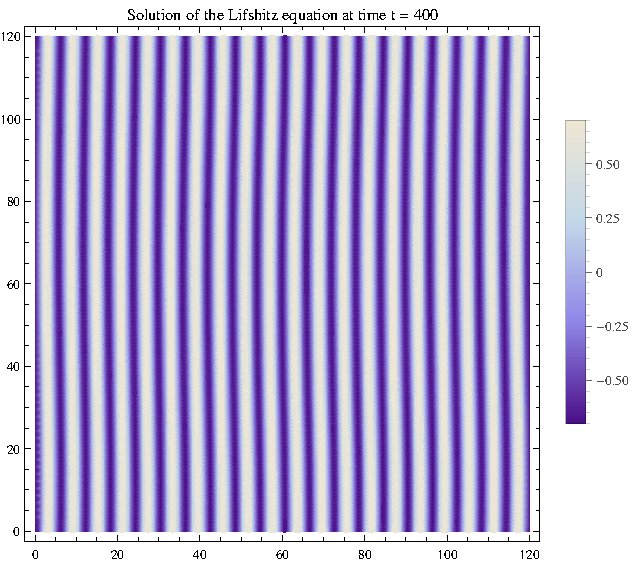
\includegraphics[scale=\scaleOne]{img/sol_Lif_t400.png}\hfill%
\end{figure} 
}

\only<1-4>{
Modèle de Lifshitz : champ $\phi(x)$ à $n$ composantes, \textcolor{BrickRed}{anisotrope}. \\
Phase de Lifshitz : $\phi(x)$ \textcolor{BrickRed}{périodique} dans $m$ directions de l'espace de dimension $d$.
}

\end{frame}

\begin{frame}

\begin{columns}

\begin{column}{5.5cm}
\begin{block}{Intérêt expérimental}

Description de nombreux systèmes : cristaux magnétiques (MnP), ferroélectriques, cristaux organiques (TTF-TCNQ),...

\end{block}
\end{column}

\begin{column}{5.5cm}
\begin{block}{Intérêt théorique}
Un exemple de système anisotropique ``fort'' : les exposants critiques dépendent de la direction.
\end{block}
\end{column}

\end{columns}

\end{frame}

\begin{frame}

\begin{block}{Hamiltonien de Lifshitz}
\centering
$ H[\phi] = \int_x  \frac{1}{2}(\p{\perp} \phi)^2 + \frac{\rho_0}{2}(\p{\sslash}\phi)^2 + \frac{\sigma_0}{2} (\p{\sslash}^2 \phi)^2 + U(\rho) \text{,~} \rho \define \frac{\phi^2}{2}$
\end{block}

\begin{figure}[htp]
\centering
\includegraphics[scale=0.65]{img/phase_diagram.pdf}
\label{}
\end{figure}

En champ moyen $\rho^{\text{Lif}}_0 = 0$ $\rightarrow$ \textcolor{BrickRed}{ajout d'un terme d'ordre $\partial_\sslash^4$}.

\end{frame}

\section{Le groupe de renormalisation non perturbatif}
\subsection{L'idée de la renormalisation}


\begin{frame}

\centering 
Problème à $N$ corps $\rightarrow$ fluctuations à toutes les échelles

Renormalisation : considérer le problème échelle par échelle.

\begin{figure}[htp]
\centering
\begin{subfigure}{.25\textwidth}
	\centering
	\includegraphics[width=.9\linewidth]{img/renorm_step0.pdf}
	\caption{Réseau initial}
	\end{subfigure}%
\begin{subfigure}{.25\textwidth}
	\centering
	\includegraphics[width=.9\linewidth]{img/renorm_step1.pdf}
	\caption{Blocs de spin}
\end{subfigure}%
\begin{subfigure}{.25\textwidth}
	\centering
	\includegraphics[width=.9\linewidth]{img/renorm_step2.pdf}
	\caption{Moyennage}
\end{subfigure}%
\begin{subfigure}{.25\textwidth}
	\centering
	\includegraphics[width=.9\linewidth]{img/renorm_step3.pdf}
	\caption{Rescaling}
\end{subfigure}
%\caption{The renormalization procedure illustrated. Here we have chosen $S = 3$.}
\label{fig:renorm_proc}
\end{figure}

\[ \textcolor{BrickRed}{H[\phi(x_i)]} \rightarrow \tilde H [\tilde{\phi}(x_b)]  \rightarrow \left.\begin{aligned}
        x' = x/S \\
        \phi' = S^\Delta \phi
       \end{aligned}
 \right\}
  \textcolor{BrickRed}{H'[\phi'(x'_i)]} \]
  
  
 \centering 
 $H'[\phi']$ : décrit le système à l'échelle $\lambda = 3 a$.
\end{frame}

\subsection{Flots et exposants critiques}
\begin{frame}
\only<1>{
\begin{figure}[htp]
\centering
\includegraphics[scale=0.4]{img/flot.pdf}
\label{}
\end{figure}

\centering
$T=T_c$ (et $\rho_0 = \rho_{0c}$) $\rightarrow$ \textcolor{BrickRed}{point fixe} sur la surface critique\\
Voisinage du point fixe : lois d'échelle $\rightarrow$ exposants critiques
\[
H[\phi] = \sum_{i, \alpha} \kappa_\alpha O_\alpha[\phi(x_i), \nabla \phi(x_i), ...] \rightarrow H'[\phi'] = \sum_{i', \alpha} \kappa_\alpha' O_\alpha[\phi'(x_i'), ...]
\]
}
\end{frame}

\subsection{Application au modèle de Lifshitz en champ moyen}
\begin{frame}

\begin{figure}[htp]
\centering
\includegraphics[scale=0.4]{img/blockspin_theta.pdf}
\label{}
\end{figure}
\begin{center}
Blocs de spin avant et après introduction de $\theta$.
\end{center}

\begin{block}{}
Directions inéquivalentes $\implies$ échelles inéquivalentes $S_\sslash$, $S_\perp$. \newline On introduit $\theta$ tel que $S_\sslash = S_\perp^\theta$. 
\end{block} 

\begin{block}{Résultats du champ moyen}
\centering
$\theta_\text{cm} = \frac{1}{2}$, $d_c^> = 4 + \frac{m}{2}$
\end{block}
\end{frame}

\subsection{Le groupe de normalisation non perturbatif}
\begin{frame}

Équation de Wetterich : évolution exacte de $\gam_k[\phi]$, action effective à l'échelle $k \propto S^{-1}$.

\begin{columns}

\begin{column}{6cm}
\begin{figure}[htp]
\centering
\includegraphics[scale=0.825]{img/propagateur.pdf}
\label{}
\end{figure}
\end{column}

\begin{column}{6cm}
\begin{figure}[htp]
\centering
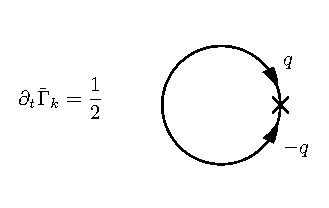
\includegraphics[scale=0.825]{img/dtgam.eps}
\label{}
\end{figure} 
\end{column}

\end{columns}

\begin{columns}

\begin{column}{6cm}
\[G_k(q_1,q_2 ; \phi) =  \left( \Gamma^{(2)}_k[\phi] + R_k \right)^{-1}_{q_1,q_2} \] 

\end{column}

\begin{column}{6cm}
\[\p{k} \gam_k[\phi] = \frac{1}{2} \int_q \p{k}R_k(q)  G_k(q,-q;\phi)  \] 
\end{column}

\end{columns}

\end{frame}

\section{Le point critique de Lifshitz : méthodes et résultats}
\subsection{L'Ansatz pour l'action effective du modèle}
\begin{frame}

\centering
$ H[\phi] = \int_x  \frac{1}{2}(\p{\perp} \phi)^2 + \frac{\rho_0}{2}(\p{\sslash} \phi)^2 + \frac{\sigma_0}{2} (\p{\sslash}^2 \phi)^2 + U(\rho)$

\begin{block}{Symétries $\implies$ forme générale de l'action effective de Lifshitz :}
$\Gamma_k[\phi] = \int_{x} U(\rho) + \frac{1}{2} Z_\perp(\rho) (\partial_\perp \phi)^2 + \frac{1}{4} Y_\perp(\rho) (\partial_\perp \rho)^2 + ... $\\
\hfill$+~ \frac{1}{2} \rho_0(\rho) (\partial_\sslash \phi)^2 + ...  +  \frac{1}{2} Z_\sslash(\rho) (\partial_\sslash^2 \phi)^2 + ... $
\end{block}

Pour calculer les exposants critiques la structure impulsionnelle importe peu $\rightarrow$ simplifications.

\begin{block}{Forme définitive de l'Ansatz :}
$\Gamma_k[\phi_i] = \int_x  \frac{Z_\perp}{2} (\partial_\perp \phi)^2 + \frac{\rho_0}{2} (\partial_\sslash \phi)^2 + \frac{Z_\sslash}{2} (\partial_\sslash^2 \phi)^2 + U(\rho).$
\end{block}

Prise en compte de \textcolor{BrickRed}{potentiel complet}.
\end{frame}

\subsection{Flots de renormalisation}
\begin{frame}

\begin{block}{Équations de flot du modèle}
\begin{itemize}
\item $k \partial_k u_k(\rho) = -d_m u_k(\rho) + (\theta \eta_\sslash + d_m - 4 \theta) \rho u_k'(\rho)$ \\
\hfill $+~8 v_m v_{d-m} \left( l_0^{dm}\left(u_k'(\rho) + 2 \rho u_k''(\rho) \right) + (n-1)l_0^{dm}\left(u_k'(\rho)\right) \right)$
\phantom{sdsldk}
\item $k \partial_k \rho_0 = -\theta \left(2-\eta_\sslash\right) \rho_0 - 64 \frac{ v_{d-m} v_m}{m} \rho u^{(2)}(\rho)^2 m_{1,2202} $

%\item $\eta_\perp = 32 v_{d-m} v_m \rho u^{(2)}(\rho)^2  m_{1,2202}$

%\item $\eta_\sslash = \eta_\perp  \Big[ m_{1,3100} - \frac{1}{2} k_{1,2100}-\frac{2}{m}\left( 6 s_{1,4102}-6 v_{1,31002}+ w_{1,2102} \right)$ \\
%\hfill$+~\frac{2}{m(m+2)}\big( 24 t_{1,5104} -36 z_{1,4104}+6 u_{1,3104} +8 y_{1,3104} - x_{1,2104} \big) \Big]$
\end{itemize}
\end{block}

Approximation du potentiel local : $\theta \simeq \theta_{\text{cm}} = \frac{1}{2}$, $\eta_{\sslash, \perp} \simeq \eta_{\text{cm}} = 0$.

\begin{block}{}
Voisinage du point de Lifshitz $\rightarrow$ résolution des \textcolor{BrickRed}{équations de point fixe} : $\p{k} u = 0$, $\p{k}\rho_0 = 0$.
\end{block}

\end{frame}

\subsection{Le potentiel au point de Lifshitz}

\begin{frame}
%\begin{block}{}
%$ 0 = -d_m u_t(\rho) + (\theta \eta_\sslash + d_m - 4 \theta) \rho u_t'(\rho)$ \\
%\hfill $+~8 v_m v_{d-m} \left( l_0^{dm}\left(u_t'(\rho) + 2 \rho u_t''(\rho) \right) + (n-1)l_0^{dm}\left(u_t'(\rho)\right) \right)$
%\end{block}

\begin{block}{Équations de point fixe :}
\begin{itemize}
\item $0 = u(\rho) - a  \rho u'(\rho) + b(\rho_0) \left( \frac{1}{1 + \rho_0 + u'(\rho) + 2 \rho u''(\rho)} + \frac{n-1}{1+\rho_0+u'(\rho)} \right)$ \\
\phantom{ddfdf}
\item $\rho_0 = 64 \frac{ v_{d-m} v_m}{m} \rho u^{(2)}(\rho)^2 m_{1,2202} $ \\
\end{itemize}
\end{block}

Conditions initiales :\\
$u'(0) = \sigma$ \\
$u\phantom{'}(0) = n b(\rho_0)/(1+\sigma)$

\begin{block}{}
Singularité à $\rho_\text{sing}(\sigma)<\infty$, sauf si $\sigma = \sigma_c$, \textcolor{BrickRed}{température critique}.
\end{block}

%\begin{block}{Stratégie de résolution}
%\begin{itemize}
%\item Commencer à $d=d_c^>$ ($\sigma^\text{Lif} = 0$, $\rho^\text{Lif}_{0} = 0$).
%\item $d \rightarrow d - \delta d$. 
%\item Trouver $\sigma^\text{Lif}$.
%\item Trouver $\rho^\text{Lif}_{0}$.
%\item Revenir à l'étape (2).
%\end{itemize}
%\end{block}

\end{frame}

\subsection{Les exposants critiques}

\begin{frame}

% modifier la taille des images de cette diapo
\newcommand{\scale}{1}

\only<1>{
\begin{figure}[htp] 
\centering
\includegraphics[scale=\scale]{img/emergence_lif_1.pdf}\hfill%
\end{figure} 
}

\only<2>{
\begin{figure}[htp] 
\centering
\includegraphics[scale=\scale]{img/emergence_lif_2.pdf}\hfill%
\end{figure} 
}

\only<3>{
\begin{figure}[htp] 
\centering
\includegraphics[scale=\scale]{img/emergence_lif_3.pdf}\hfill%
\end{figure} 
}

\only<4>{
\begin{figure}[htp] 
\centering
\includegraphics[scale=\scale]{img/emergence_lif_4.pdf}\hfill%
\end{figure} 
}

\only<5>{
\begin{figure}[htp] 
\centering
\includegraphics[scale=\scale]{img/emergence_lif_5.pdf}\hfill%
\end{figure}
}

\only<1-5>{
\centering
Position de la singularité $\rho_\text{sing}$ en fonction de la condition initiale $\sigma$.
}
\end{frame}

\subsection{Flot du potentiel}
\begin{frame}



\begin{columns}

\begin{column}{6cm}
\begin{figure}[htp]
\centering
\includegraphics[scale=0.45]{img/plotflowd3.pdf}
\label{}
\end{figure}
\end{column}

\begin{column}{6cm}
\begin{figure}[htp]
\centering
\includegraphics[scale=0.45]{img/plotlogflowd3.pdf}
\label{}
\end{figure}
\end{column}

\end{columns}

\[
\begin{aligned}
u_t(\rho)  &= u(\rho) + \delta u_\sslash(\rho) e^{t/\nu_\sslash} + \delta u_\perp(\rho) e^{t/\nu_\perp} \\
t &\define \log k
\end{aligned}
\]

\begin{center}
\label{tab:results}
\begin{tabular}{|c|c|c|c|}
\hline 
\rule[-1ex]{0pt}{2.5ex} ~ & nos résultats & dév. perturbatif & Wilson-Polchinski \\ 
\hline 
\rule[-1ex]{0pt}{2.5ex} $\nu_\sslash$ & 0.399 & 0.392 & 0.317 \\ 
\hline 
\rule[-1ex]{0pt}{2.5ex} $\nu_\perp$ & 0.799 & 0.798 & 0.634 \\ 
\hline 
\end{tabular} 
\end{center}


\end{frame}

\section{Conclusion}
\begin{frame}

\begin{itemize}
\item Calcul des exposants critiques d'un modèle non trivial, par une méthode originale.
\item Prise en compte du potentiel complet.
\item Prochain objectif : prise en compte des dimensions anormales.
\end{itemize}

\end{frame}

\end{document}